%! Author = verwoerd
%! Date = 9-8-2023

% Preamble
\documentclass[11pt,pdf, aspectratio=169]{beamer}
\usetheme{metropolis}
\title{DAPC 2023 Training Sessions\\Session 2}
\date{September 18, 2023}
\author{Verwoerd}

% Packages
\usepackage{amsmath}
\usepackage{amssymb}
\usepackage[utf8]{inputenc}
\usepackage[T1]{fontenc}
\usepackage{graphicx}
\usepackage{tikz}
\usepackage{minted}
\usepackage[
  type={CC},
  modifier={by-sa},
  version={4.0},
]{doclicense}
\usepackage{hyperref}
\setsansfont{Fira Sans}
\usemintedstyle{manni}
\setminted{
  fontsize=\footnotesize,linenos,frame=lines, framesep=2mm
}
\usetikzlibrary{angles,quotes,graphs, graphdrawing}
\usegdlibrary {layered}

% Document
\begin{document}
  \maketitle
  \begin{frame}{Session 2}
    \begin{itemize}
      \item Team Tactics
      \item Utilizing the Test Session
      \item How to select problems
      \item Solutions to the Ad-hoc and Math Problems
      \item Solving Sorting and Search Problems
    \end{itemize}
    \doclicenseThis
  \end{frame}


  \section{Team Tactics}
  \begin{frame}{General Tactics}
    \begin{itemize}
      \item Know each other's strengths and weaknesses like:
      \begin{itemize}
        \item types of problems (math, geometry, search, strings, graphs, etc.)
        \item debugging skills
        \item coding speed and accuracy
      \end{itemize}
      \item Parallelize
      \item Work on paper (e.g. pseudocode or flow diagrams)
      \item Debug on paper
      \item Use rubber duck debugging when stuck
    \end{itemize}
  \end{frame}
  \begin{frame}{Team Tactics}
    \begin{itemize}
      \item<1-> Plot of the contest: 3 contestants, 1 computer
      \item<2-> Several tactics how to divide the computer efficiently
      \item<3-> Shuffle Tactic\begin{itemize}
                                \item<4-> Rotate around who sits behind the pc
                                \item<4-> After submitting a problem, switch around if someone has a solution
                                \item<4-> Useful when programming in different languages
      \end{itemize}
      \item<3-> Designated Tactic\begin{itemize}
                                   \item<5->Dedicated person behind computer
                                   \item<5-> Other team members work on paper or read along on screen
                                   \item<5-> Useful for teams with different disciplines
      \end{itemize}
      \item<3-> No best solution: Pick and mix what works best for your team
    \end{itemize}
  \end{frame}
  \begin{frame}{Common Battle Plan}
    \begin{description}
      \item [Start of contest] Prepare computer, find and solve easiest problems, all problems should be read by at least a single team member.
      \item[First hours] Prioritize solving the easiest problems, every team member works on their own problems
      \item[Mid contest] Work on solving harder problems with 2 people, while the last person works alone on the last easy or specialized hard problems
      \item[End of the contest] Work together with the whole team on a single problem, free submit mode
    \end{description}
  \end{frame}
  \begin{frame}{Common Errors}
    \begin{itemize}
      \item Focus on the first problem you think you can solve
      \item Not reading all problems in the set
      \item Debugging on the computer while another solution can be implemented
      \item Fighting who can solve which problem
      \item Not rewriting code when it gets to messy
    \end{itemize}
  \end{frame}


  \section{Utilizing the Test Session}
  \begin{frame}{Utilizing the Test Session}
    \begin{itemize}
      \item The test session is a short version practice contest with a few simple problems
      \item Find your team workspace
      \item Practice start of the contest, e.g. where are the problems located, how is the start announced
      \item Practice end of the contest, e.g. freeze warning, countdown.
    \end{itemize}
  \end{frame}
  \begin{frame}{Testing the envirionment}
    \begin{itemize}
      \item<1-> Get to know the programming environment and its quirks
      \item <2-> Where is everything located: samples, documentation, important links
      \item <3-> Try all IDE and tools you \textit{might} use during the contest
      \item <4-> Test out printing, if supported, from IDE, command line, and CCS
      \item <5-> All files will be removed after the test session!
    \end{itemize}
  \end{frame}
  \begin{frame}{Testing the Contest System}
    \begin{itemize}
      \item Test the possible problems, how are they reported back
      \begin{itemize}
        \item Correct (AC)
        \item Wrong Answer (WA)
        \item Run Time Error (RTE), like segmentation fault, going over heap/stack space, null pointer exception, array index out of bounds
        \item Time Limit Exceeded (TLE)
        \item Compiler Error
      \end{itemize}
      \item Test clarification requests
      \item Where are general clarifications displayed
    \end{itemize}
  \end{frame}


  \section{Hints on selecting the problems}
  \begin{frame}{Selecting the first problem}
    \begin{itemize}
      \item Decide on a reading tactic
      \begin{itemize}
        \item Do we all start reading the first problem?
        \item Or does one person start at the end?
      \end{itemize}
      \item There are usually several ``simple'' problems in a set
      \item Be careful: the easiest problems usually contain some pitfall corner cases!
    \end{itemize}
  \end{frame}
  \begin{frame}{Finding the easiest problems by results}
    \begin{itemize}
      \item After a few minutes of contest, the first balloons will be handed out
      \item Check the scoreboard or balloon colours to see which problem is solved most\\
      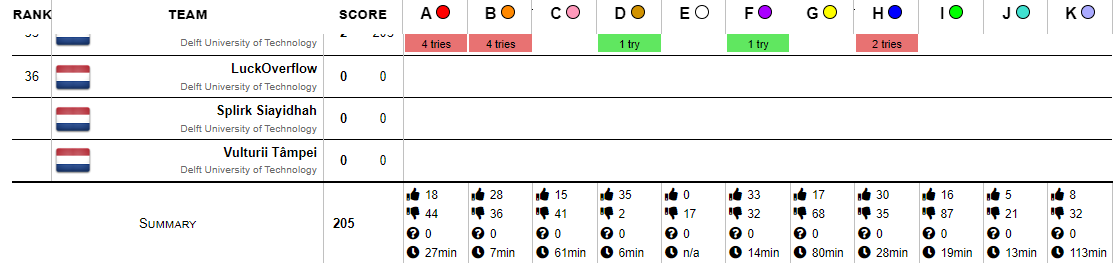
\includegraphics[width=\linewidth]{images/session-2/bottom-scoreboard}
      \item Or the problems page in DOMJudge (only newer versions)
      \item \textbf{Warning}: The first problem solved is not guaranteed the easiest!
    \end{itemize}
  \end{frame}
  \begin{frame}{My problem is wrong, what now}
    Print out the problem and let other people work on the computer, work out cases that might go wrong.
    \begin{itemize}
      \item When the result is RTE:
      \begin{itemize}
        \item Check for possible null pointers, array overflows, or integer overflow
        \item Check the input specification, don't forget 0 can do unexpected things
      \end{itemize}
      \item When the result is TLE:
      \begin{itemize}
        \item Check stop conditions, maybe an infinite loop?
        \item Code is too slow, try optimizing or thinking of a faster solution
      \end{itemize}
      \item When then result is WA:
      \begin{itemize}
        \item Check for corner cases, don't forget zero
        \item Check correctness of algorithm
      \end{itemize}
      \item \textbf{Warning}: A problem can be WA and TLE at the same time, but only \emph{one} is reported back!
    \end{itemize}
  \end{frame}


  \section{Solutions to the ad-hoc and math problems}
  \begin{frame}{Jabbing Jets}
    \begin{itemize}
      \item Source BAPC Preliminaries 2022
      \item Time limit: 1s
      \item Given $n$ concentric circles, find the maximal number of points on these circles such that the distance between any two points is at least $e$.
    \end{itemize}
    Original problem written by the BAPC 2022 jury and licensed under \doclicenseLongNameRef.

    \doclicenseImage

  \end{frame}
  \begin{frame}{Jabbing Jets}
    \begin{columns}
      \column{0.75\textwidth}
      \begin{itemize}
        \item<1-> Observation 1: $n \leq 10^4$ and time limit of 1s so looking for $\mathcal{O}(n)$ solution
        \item<2-> Observation 2: Because $r_{i+1}-r_i \geq e$ every circle can be considered separately.
        \item<3-> 2 points are divided by angle $\alpha$
        \item<3-> You can calculate $\alpha = 2 \arcsin{}(\frac{e}{2r})$
        \item<4-> The radius of a circle is $2\pi$ so the max number of points with distance $e$ can be calculated by\\
        $\left\lfloor\frac{2\pi}{\alpha}\right\rfloor \equiv \left\lfloor \frac{2\pi}{2 \arcsin{}(\frac{e}{2r})}\right\rfloor$
        \item<5-> Do this for every circle and sum the numbers
        \item<5-> Pitfall 1: if $2r < e$ then there can only be one point
        \item<5-> Pitfall 2: rounding can cause issues, add $0.5\cdot 10^{-6}$
      \end{itemize}
      \column{.25\textwidth}
      \input{dapc-j.tikz}
    \end{columns}
  \end{frame}
  \begin{frame}[containsverbatim]{Solution for Jabbing Jets}
    \inputminted{python}{code/session-1/python/dapc-j.py}
  \end{frame}
  \begin{frame}{Lots of Liquid}
    \begin{itemize}
      \item Source BAPC Preliminaries 2022
      \item Time limit: 1s
      \item Find the length of the side of a cube that contains all liquid.
    \end{itemize}
    Original problem written by the BAPC 2022 jury and licensed under \doclicenseLongNameRef.

    \doclicenseImage
  \end{frame}
  \begin{frame}{Lots of Liquid}
    \begin{itemize}
      \item<1-> Observation: $n \leq 10^5$, so we are looking for a $\mathcal{O}(n)$ solution
      \item<2-> The volume of a cube is $c^3$
      \item<3-> The length of cube with volume v is $\sqrt[3]{v}$
      \item<4-> Sum all volumes of the cubes and calculate the length of the cube
      \item<4-> Print out \[\sqrt[3]{\sum_{i=1}^nc_i}\]
    \end{itemize}
  \end{frame}
  \begin{frame}[containsverbatim]{Lots of Liquid}
    \inputminted{python}{code/session-1/python/dapc-l.py}
  \end{frame}
  \begin{frame}{Bellevue}
    \begin{itemize}
      \item Source BAPC 2022
      \item Time limit: 1s
      \item  Given the profile of an island, find the point with the largest viewing angle of the sea.
    \end{itemize}
    Original problem written by the BAPC 2022 jury and licensed under \doclicenseLongNameRef.

    \doclicenseImage
  \end{frame}
  \begin{frame}{Bellevue}
    \begin{itemize}
      \item<1-> The answer is always an angle from the start or the end of the island to another point
      \item<2-> Calculate the angle from start and end to any other point
      \item<2-> Print out the solution
      \item<3-> Alternatively, calculate the convex hull
      \begin{itemize}
        \item<3-> The best angle is from either the first and second point in the hull or the last and previous
      \end{itemize}
    \end{itemize}
  \end{frame}
  \begin{frame}[containsverbatim]{Bellevue}
    \inputminted{python}{code/session-1/python/bapc-b.py}
  \end{frame}
  \begin{frame}{Equalising Audio}
    \begin{itemize}
      \item Source BAPC 2022
      \item Time limit: 4s
      \item  Given a list of frequencies, normalize it so the perceived loudness is \[\frac{1}{n} \sum^n_{i=1}a_i^2=x\]
    \end{itemize}
    Original problem written by the BAPC 2022 jury and licensed under \doclicenseLongNameRef.

    \doclicenseImage
  \end{frame}
  \begin{frame}{Equalising Audio}
    \begin{itemize}
      \item<1-> Observation: time limit is high for I/O operations
      \item<2-> First calculate the current perceived loudness \[x_{cur} = \frac{1}{n} \sum^n_{i=1}a_i^2\]
      \item<3-> Then print out the frequency reduced by $\sqrt{\frac{x}{x_{cur}}}$, since
      \[\frac{1}{n} \sum^n_{i=1}\left(\sqrt{\frac{x}{x_{cur}}}a_i\right)^2 = \frac{1}{n} \sum^n_{i=1}\left(\sqrt{\frac{x}{x_{cur}}}\right)^2a_i^2 = \frac{x}{x_{cur}}\cdot \frac{1}{n}\sum^n_{i=1}a_i^2 = \frac{x}{x_{cur}}\cdot x_{cur} = x\]
      \item<4-> Pitfall: if the current perceived loudness ($x_{cur}$) is 0, the result is \texttt{0 0 \ldots{} 0}
    \end{itemize}
  \end{frame}
  \begin{frame}[containsverbatim]{ Equalising Audio}
    \inputminted{python}{code/session-1/python/bapc-e.py}
  \end{frame}
  \begin{frame}{Failing Flagship}
    \begin{itemize}
      \item Source BAPC 2022
      \item Time limit: 1s
      \item  Compute the minimum angle in degrees between two wind directions.
    \end{itemize}
    Original problem written by the BAPC 2022 jury and licensed under \doclicenseLongNameRef.

    \doclicenseImage
  \end{frame}
  \begin{frame}{Failing Flagship}
    \begin{itemize}
      \item<1-> Convert the letters to degrees $d_1$ and $d_2$
      \item<2-> Execute the algorithm as described in the problem by adding and subtracting a delta, starting at $45\deg$
      \item<3-> Every next letter represents a half of previous delta and either add or subtract it
      \item<4-> Be careful of overflow with NW
      \item<4-> Print out $\min(d_2-d_1, 360+d_1-d_2)$
    \end{itemize}
  \end{frame}
  \begin{frame}[containsverbatim]{Failing Flagship}
    \inputminted{python}{code/session-1/python/bapc-f.py}
  \end{frame}


  \section{Solving Sorting and Search Problems}
  \begin{frame}{Natural Order Sorting Algorithms}
    \begin{itemize}
      \item Sorting algorithms sort items in a natural order
      \item Use built-in sort as much of possible
      \item C++17: \mintinline{c++}|std::sort()|
      \item Python: \mintinline{python}|list.sort()| or \mintinline{python}|sorted()|
      \item Java/Kotlin: \mintinline{java}|Arrays.sort()| or \mintinline{java}|Collections.sort()|
      \item C++ uses IntroSort and Python/Java/Kotlin use TimSort, both $\mathcal{O}(n\log{}n)$
      \item For special case sorting, write a specific comparator or key function (Python)
    \end{itemize}
  \end{frame}
  \begin{frame}{Binary Search}
    \begin{itemize}
      \item If the input is sorted or monotonically increasing you can use binary search
      \item Start in the middle and half the search space based on if the value is to high or to low
      \item Results in an $\mathcal{O}(\log{}n)$ algorithm
      \item C++17: \mintinline{c++}|std::binary_search()|
      \item Python: \mintinline{python}|bisect.bisect()|
      \item Java/Kotlin: \mintinline{java}|Arrays.binarySearch()| or \mintinline{java}|Collections.binarySearch()|
      \item Implementing your own binary search is error prone!
    \end{itemize}
  \end{frame}
  \begin{frame}{Depth first search (DFS)}
    \begin{columns}
      \column{.66\textwidth}
      \begin{itemize}
        \item Greedy algorithm to search a graph or tree
        \item Visit every node when it is discovered
        \item Usually implemented by using a stack data structure
        \item Use an array to keep track of discovered nodes
        \item Example application is solving a maze
        \item \textbf{Note}: Using a boolean array is faster then using a set
      \end{itemize}
      \column{.34\textwidth}
      \begin{tikzpicture}
        \graph[layered layout] {
          a -- b -- d;
          b -- e;
          a -- c -- f;
          c -- g;
        };
      \end{tikzpicture}\\
      DFS Traverses the path
      \begin{tikzpicture}
        \graph[layered layout] {
          1 -- 2 -- 3;
          2 -- 4;
          1 -- 5 -- 6;
          5 -- 7;
        };
      \end{tikzpicture}\\
      resulting order: a b d e c f g
    \end{columns}
  \end{frame}
  \begin{frame}{Breath first search (BFS)}
    \begin{columns}
      \column{.66\textwidth}
    \begin{itemize}
      \item Similar to DFS, but visits based on discovery order
      \item Usually implemented using a queue
      \item Example application is flood-filling to find a closest node
    \end{itemize}
      \column{.34\textwidth}
      \begin{tikzpicture}
        \graph[layered layout] {
          a -- b -- d;
          b -- e;
          a -- c -- f;
          c -- g;
        };
      \end{tikzpicture}\\
      DFS Traverses the path
      \begin{tikzpicture}
        \graph[layered layout] {
          1 -- 2 -- 4;
          2 -- 5;
          1 -- 3 -- 6;
          3 -- 7;
        };
      \end{tikzpicture}\\
      resulting order: a b c d e f g
    \end{columns}
  \end{frame}
  \begin{frame}{Search using a heap}
    \begin{itemize}
      \item Search a space, selecting the next position by a condition
      \item For example: the closest discovered node in Dijkstra's Shortest Path Algorithm
      \item C++17: \mintinline{c++}|std::priority_queue|
      \item Python: \mintinline{python}|heapq.heapify()|
      \item Java/Kotlin: \mintinline{java}|java.util.PriorityQueue()|
    \end{itemize}
  \end{frame}
  \begin{frame}{Problem: Bubble-bubble Sort}
    \begin{itemize}
      \item Source BAPC Preliminaries 2022
      \item Problem name: Bubble-bubble Sort
      \item Time limit: 2s
    \end{itemize}
    Original problem written by the BAPC 2022 jury and licensed under \doclicenseLongNameRef.

    \doclicenseImage

  \end{frame}
  \begin{frame}{Problem: Bubble-bubble Sort (1)}
    Bubbles!
    As a fanatical supporter of the Bubbles Are Perfect Creatures movement, you have accumulated a large collection of bubbles in all colours and sizes.
    Being a long time member, your bubbles are among the best in the world, and now is the time to show this.
    Tomorrow, the yearly Bubble Exposition will be held, and your goal is to win the Bubble Prize and become the Bubble Champion!

    However, this is not an easy competition.
    In order to win, you do not only need the most beautiful bubbles, you also need the best-looking placement of bubbles.
    You have decided to order the bubbles by bubbliness: less bubblier bubbles to the left, more bubblier bubbles to the right.
    However, it is hard to compare all the bubbles in your collection at once. In fact, you can only compare up to $k$ bubbles by eye before losing track of all the bubbles.
    Since your collection consists of more than $k$ bubbles, you need a fancier sorting algorithm.


  \end{frame}
  \begin{frame}{Problem: Bubble-bubble Sort (2)}
    Your first thought is to use the best sorting algorithm for bubbly purposes, namely Bubble Sort.
    However, this is the most prestigious bubble competition, so you decide to do better: Bubble-bubble Sort. It works as follows.

    Initially, your bubbles are placed in an arbitrary order.
    Every hour, you do the following: you look at the first $k$ bubbles and place them in the optimal order.
    Then, you look at bubbles $2$ to $k+1$ and place those in the correct order.
    Then, you look at bubbles $3$ to $k+2$, and so on, until you have placed the last $k$ bubbles in the correct order.
    You then admire how the bubble collection looks so far until the next hour begins and you start at the first bubbles again.

    Is this algorithm fast enough to place all your bubbles, or do you need to go further and invent a Bubble-bubble-bubble Sort algorithm?
    To be precise, after how many hours are the bubbles in the optimal positions?
  \end{frame}
  \begin{frame}{Problem: Bubble-bubble Sort: Input and Output}
    \textbf{Input}
    The input consists of:
    \begin{itemize}
      \item One line with two integers $n$ and $k$ ($2 \leq k < n \leq 2500$), the number of bubbles and the number of bubbles you can sort at once.
      \item One line with $n$ integers $a$ ($0 \leq a \leq 10^9$), the bubbliness of each bubble in the initial placement of your bubble collection.
    \end{itemize}

    \textbf{Output}

    Output the number of hours needed to sort your bubble collection.
  \end{frame}
  \begin{frame}{Problem: Bubble-bubble Sort: Samples}
    \begin{tabular}{|l|l|}
      \hline
      \textbf{Sample Input 1} & \textbf{Sample Output 1} \\
      \hline
      \texttt{5 2}            & \texttt{3}               \\
      \texttt{3 4 1 5 2}      &                          \\
      \hline
    \end{tabular}

    \begin{tabular}{|l|l|}
      \hline
      \textbf{Sample Input 2}        & \textbf{Sample Output 2} \\
      \hline
      \texttt{8 3}                   & \texttt{2}               \\
      \texttt{60 8 27 7 68 41 53 44} &                          \\
      \hline
    \end{tabular}

    \begin{tabular}{|l|l|}
      \hline
      \textbf{Sample Input 3} & \textbf{Sample Output 3} \\
      \hline
      \texttt{6 3}            & \texttt{3}               \\
      \texttt{3 2 4 2 3 1}    &                          \\
      \hline
    \end{tabular}
  \end{frame}
  \begin{frame}{Problem: Bubble-bubble Sort: Example 2: After 1 hour}
    Window $k$ is 3.\\
    \begin{tabular}{|l|rrrrrrrr|}
      \hline
      Hour   &    &    &             &             &    &    &             &             \\
      \hline
      0      & 60 & 8  & 27          & 7           & 68 & 41 & 53          & 44          \\
      \hline
      step 1 & 8  & 27 & 60          &             &    &    &             &             \\
      step 2 &    & 7  & 27          & 60          &    &    &             &             \\
      step 3 &    &    & 27          & 60          & 68 &    &             &             \\
      step 4 &    &    &             & 41          & 60 & 68 &             &             \\
      step 5 &    &    &             &             & 53 & 60 & 68          &             \\
      step 6 &    &    &             &             &    & 44 & 60          & 68          \\
      \hline
      hour 1 & 8  & 7  & \textbf{27} & \textbf{41} & 53 & 44 & \textbf{60} & \textbf{68} \\
      \hline
    \end{tabular}\\
    List is not sorted yet, we need an other hour.
  \end{frame}
  \begin{frame}{Problem: Bubble-bubble Sort: Example 2: After 2 hours}
    Window $k$ is 3.\\
    \begin{tabular}{|l|rrrrrrrr|}
      \hline
      Hour   &   &   &    &    &    &    &    &    \\
      \hline
      hour 1 & 8 & 7 & 27 & 41 & 53 & 44 & 60 & 68 \\
      \hline
      step 1 & 7 & 8 & 27 &    &    &    &    &    \\
      step 2 &   & 8 & 27 & 41 &    &    &    &    \\
      step 3 &   &   & 27 & 41 & 53 &    &    &    \\
      step 4 &   &   &    & 41 & 44 & 53 &    &    \\
      step 5 &   &   &    &    & 44 & 53 & 60 &    \\
      step 6 &   &   &    &    &    & 53 & 60 & 68 \\
      \hline
      hour 2 & 7 & 8 & 27 & 41 & 44 & 53 & 60 & 68 \\
      \hline
    \end{tabular}\\
    List is sorted, so solution is 2.
  \end{frame}
  \begin{frame}{Problem: Bubble-bubble Sort: Naive Solution}
    \begin{itemize}
      \item<1-> Observation: $n \leq 2500$, so the target is an $\mathcal{O}(n^2)$  solution
      \item<2-> Worst case is described in example 3:\\
      \begin{tabular}{|l|rrrrrr|}
        \hline
        hour 0 & 3          & 2          & 4 & 2          & 3 & \textbf{1} \\
        \hline
        hour 1 & 2          & 2          & 3 & \textbf{1} & 3 & 4          \\
        hour 2 & 2          & \textbf{1} & 2 & 3          & 3 & 4          \\
        \hline
        hour 3 & \textbf{1} & 2          & 2 & 3          & 3 & 4          \\
        \hline
      \end{tabular}
      \item<3-> The lowest number is at the right most position and moves $k-1$ steps to the left, while total steps needed are $n-1$.
      \item<3-> So the worst case number of hours is $\left\lceil\frac{n-1}{k-1}\right\rceil$
      \item<4-> The described algorithm is $\mathcal{O}\left(\frac{n-1}{k-1}n\right) \simeq \mathcal{O}(n^2)$
    \end{itemize}
  \end{frame}
  \begin{frame}{Problem: Bubble-bubble Sort: Smart Solution}
    \begin{itemize}
      \item<1-> First sort the list to determine the new position of each item $a_i$.
      \item<1-> Warning: Be mindful of duplicates, link the indexes
      \item<2-> Then print out with $i$ is the index of the input
      \[\max D_i = \begin{cases}
                     1 & \text{if } i < a_i \text{ (The item moves right)}\\
                     0 & \text{if } i = a_i \text{ (The item is in the correct position)}\\
                     \left\lceil\frac{i-a_i - 1}{k-1}\right\rceil & \text{(the item moves left)} \\
      \end{cases}\]
      \item<3-> The complexity is $\mathcal{O}(n\log{}n)$ (sorting) + $\mathcal{O}(n)$ (finding the max $D_i$)
    \end{itemize}
  \end{frame}
  \begin{frame}[containsverbatim]{ Problem: Bubble-bubble Sort: Solution}
    \inputminted{python}{code/session-1/python/dapc-b.py}
  \end{frame}
  \begin{frame}{Problem: Imperfect Imperial Units}
    \begin{itemize}
      \item Source BAPC 2022
      \item Problem name: Imperfect Imperial Units
      \item Time limit: 4s
    \end{itemize}
    Original problem written by the BAPC 2022 jury and licensed under \doclicenseLongNameRef.

    \doclicenseImage
  \end{frame}
  \begin{frame}{Problem: Imperfect Imperial Units}
    You are writing a paper for the Beta Astronomy Physics Conference about your recent discovery on grey holes.
    One of your collaborators has performed a huge number of measurements,which you would like to analyse in order to draw some conclusions.
    The only problem is: the data is measured in a wide variety of units, and to your disgust, they appear to use a mix of the imperial and metric systems.
    To simplify your analysis, you need to convert all these measurements into a different unit.
  \end{frame}
  \begin{frame}{Problem: Imperfect Imperial Units: Input}
    The input consists of:
    \vspace{-0.5em}% Attempt to make everything fit in two pages
    \begin{itemize}
      \item One line with two integers $n$ and $q$ ($1\leq n\leq 100$, $1\leq q\leq 10,000$),
      the number of unit conversion equations and the number of queries to answer.
      \item $n$ lines, each defining a unit conversion in the format\\ ``\texttt{1 <unit> = <value> <unit>}''.
      \item $q$ lines, each with a query in the format ``\texttt{<value> <unit> to <unit>}''.
    \end{itemize}

    \vspace{-0.5em}% Attempt to make everything fit in two pages
    In these formats, ``\texttt{<value>}'' is a floating-point number $v$
    ($0.001 \leq v \leq 1000$, with at most $9$ digits after the decimal point) and
    ``\texttt{<unit>}'' is a string of at most $20$ English lowercase letters (\texttt{a-z}).
    A unit in a query is guaranteed to be defined in at least one unit conversion equation.
    Every unit can be converted into every other unit in \emph{at most} one way.
  \end{frame}
  \begin{frame}{Problem: Imperfect Imperial Units: Output}
    For every query, output the value of the requested unit, or ``\texttt{impossible}'' if the query cannot be answered.

    Your answers should have a \emph{relative} error of at most $10^{-6}$.

  \end{frame}
  \begin{frame}{Problem: Imperfect Imperial Units: Samples (1)}
    \begin{tabular}{|l|l|}
      \hline
      Input Sample 1               & Output Sample 1 \\
      \hline
      4 3                          &                 \\
      1 foot = 12 inch             &                 \\
      1 yard = 3 foot              &                 \\
      1 meter = 100 centimeter     &                 \\
      1 centimeter = 10 millimeter &                 \\
      750 millimeter to meter      & 0.75            \\
      42 yard to inch              & 1512            \\
      10 meter to foot             & impossible      \\
      \hline
    \end{tabular}
  \end{frame}

  \begin{frame}{Problem: Imperfect Imperial Units: Samples (2)}
    \begin{tabular}{|l|l|}
      \hline
      Input Sample 2                    & Output Sample 2           \\
      \hline
      4 3                               &                           \\
      1 fortnight = 14 day              &                           \\
      1 microcentury = 0.036525 day     &                           \\
      1 microcentury = 1000 nanocentury &                           \\
      1 week = 7 day                    &                           \\
      22.2 fortnight to nanocentury     & 8509240.2464065708427     \\
      2.5 nanocentury to week           & 1.3044642857142857142e-05 \\
      3.14 day to fortnight             & 0.22428571428571428572    \\
      \hline
    \end{tabular}
  \end{frame}

  \begin{frame}{Problem: Imperfect Imperial Units: Samples (3)}
    \begin{tabular}{|l|l|}
      \hline
      Input Sample 3                   & Output Sample 3           \\
      \hline
      10 2                             &                           \\
      1 micrometer = 1000 nanometer    &                           \\
      1 millimeter = 1000 micrometer   &                           \\
      1 meter = 1000 millimeter        &                           \\
      1 kilometer = 1000 meter         &                           \\
      1 megameter = 1000 kilometer     &                           \\
      1 lightsecond = 299.792458 meter &                           \\
      1 lightminute = 60 lightsecond   &                           \\
      1 lighthour = 60 lightminute     &                           \\
      1 lightday = 24 lighthour        &                           \\
      1 lightyear = 365.25 lightday    &                           \\
      42 nanometer to lightyear        & 4.439403502903384947e-18  \\
      42 lightyear to nanometer        & 3.9735067984839359997e+20 \\
      \hline
    \end{tabular}
  \end{frame}

  \begin{frame}{Problem: Imperfect Imperial Units: Solution}
    Create a graph from for the $n$ rules, which has max 100 nodes


    \begin{tabular}{c|c|c}
      Sample 1               & Sample 2               & Sample 3               \\
      \hline
      \input{bapc-i-s1.tikz} & \input{bapc-i-s2.tikz} & \input{bapc-i-s3.tikz} \\
    \end{tabular}
  \end{frame}

  \begin{frame}{Problem: Imperfect Imperial Units: Solution}
    \begin{itemize}
      \item For every query use use a BFS/DFS to search for a path from the first unit to the requested node
      \item The problem specification ensures at most 1 path can exist, if no path is found, print out ``impossible''
      \item This will give a $\mathcal{O}(n\cdot q)$ complexity of the algorithm
      \item This is fast enough.
    \end{itemize}
  \end{frame}
  \begin{frame}[containsverbatim]{ Problem: Imperfect Imperial Units: Solution}
    \inputminted[fontsize=\tiny]{python}{code/session-1/python/bapc-i-search.py}
  \end{frame}
  \begin{frame}{Imperfect Imperial Units: Improved Solution}
    \begin{itemize}
      \item<1-> Our solution performs duplicate calculations, since the number of queries is significantly larger then number of units.
      \item<2-> You can cache found (sub)conversions for future queries
      \item<3-> Or we can add some preprocessioning, calculating the conversion unit for every possible unit reachable
      \item<3-> There are $\frac{n(n-1)}{2}$ combinations to calculate first ($\mathcal{O}(n^2)$)
      \item<3-> Then, for every query, we can just look up the factor and calculate the difference
      \item<4-> Resulting in a faster $\mathcal{O}(n^2 + q)$
      \item<5-> \textbf{Pitfall}: The result will fit in a double, but be careful with printing precision in C++. Avoid \mintinline{c++}|std::cout << std::fixed| here!
    \end{itemize}
  \end{frame}
  \begin{frame}[containsverbatim]{ Problem: Imperfect Imperial Units: Improved Solution}
    \inputminted[fontsize=\tiny]{python}{code/session-1/python/bapc-i-cache.py}
  \end{frame}


  \section{Conclusion}
  \begin{frame}{Guest speaker}
    % ?
  \end{frame}
  \begin{frame}{Next Session}
    Next session is on Monday the 18th of September.\\

    \url{https://domjudge.ewi.tudelft.nl/}
  \end{frame}
\end{document}
